\subsubsection{Rancangan Detail Komponen Benchmark}
\label{subsubsection:detail-data-benchmark}

Komponen \textit{benchmark} bertanggung jawab untuk melakukan pengujian terhadap sistem yang telah dibangun. Pengujian ini juga bertujuan menghasilkan data analisis. Komponen \textit{benchmark} dapat mengatur variabel melalui \textit{Test Run Config}. Variabel ini kemudian digunakan untuk membuat \textit{Test Execution Loop} yang akan mengeksekusi semua kombinasi dari variabel yang telah ditentukan. Dalam setiap iterasi dari \textit{Test Execution Loop} akan membangun sistem menggunakan \textit{Process Manager}. \textit{Process Manager} akan mengelola proses sistem yang akan diuji dengan masing-masing \textit{Node} berada pada proses yang berbeda. Setelah sistem dibangun, \textit{Process Manager} akan mengirimkan perintah untuk memulai sistem dan menyimpan \textit{PID} dari setiap proses yang berjalan. Pengujian akan dilakukan dengan k6 yang akan mengirimkan \textit{request} ke sistem yang sedang diuji. Ilustrasi struktur komponen \textit{benchmark} dapat dilihat pada gambar \ref{fig:benchmark-structure}.

\begin{figure}[ht]
    \centering
    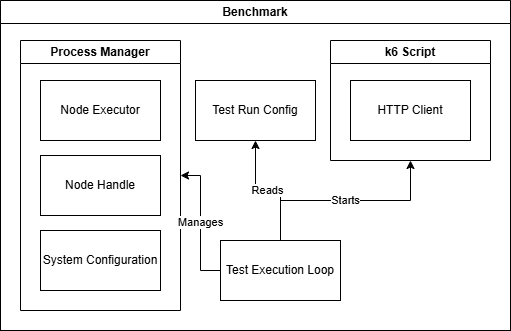
\includegraphics[width=0.55\textwidth]{resources/chapter-3/benchmark-architecture.png}
    \caption{Struktur Komponen Benchmark}
    \label{fig:benchmark-structure}
\end{figure}

Setelah pengujian selesai, manajemen \textit{node} akan mengirimkan perintah untuk menghancurkan sistem yang diuji dan membuat ulang dengan konfigurasi selanjutnya. Pengujian akan diulang hingga semua kombinasi dari variabel yang telah ditentukan selesai dieksekusi.